\section{Digital Teori}
Til dette projekt anvendes CY8CKIT-043 Programmable System on Chip (PSoC) 4 M-Series Prototyping Kit og programmet PSoC Creater i den digitale del til at opsamle det biologiske signal.\\
CY8CKIT-043 PSoC 4 M-Series Prototyping Kit er en prototyping platform, der indeholder tre mikroprocessorer: to Programmable System-on-Chips (PSoC) og en Programmable Radio on Chip (PRoC)% Advanced RISC\fxnote{REDUCED INSTRUCTION SET COMPUTER - RISK kan load/store og har pipelinable instructions, hbvilket betyder, at vi ikke behøver vente på, at en instruktion bliver færdig før vi starter med den næste. Fetch - decode - exicude, laver mere på samme tid. (kilde - slide første forelæsning)} Machines (ARM) mikroprocessorer
, hvilket ses på \figref. Den første PSoC LP5 på mikrokontrolleren kan indeholde programmer, der kan indlæses på en computer ved hjælp af USB stikket. Den bruges til at programmere og debug softwaren på programmeringsdelen af mikrokontrolleren, hvorfor denne del kan knækkes af resten af stikket og fungere selvstændigt. Dette kræver dog, at softwaren først er programmeret på den anden mikroprocessorer, som er PSoC 4200M. Denne fungerer som hovedcomputeren, der programmeres på igennem c koden. På bagsiden af mikrokontrolleren sidder en PRoC med bluetooth low energy(BLE). \fxnote{Denne PRoC har ikke lige så mange muligheder for afbenyttelse, da BLE fylder så meget, så der er ikke plads til meget andet.}\citep{CYPRESS2016PSoC,Semiconductor2016}
\begin{figure}[H]
	\centering
	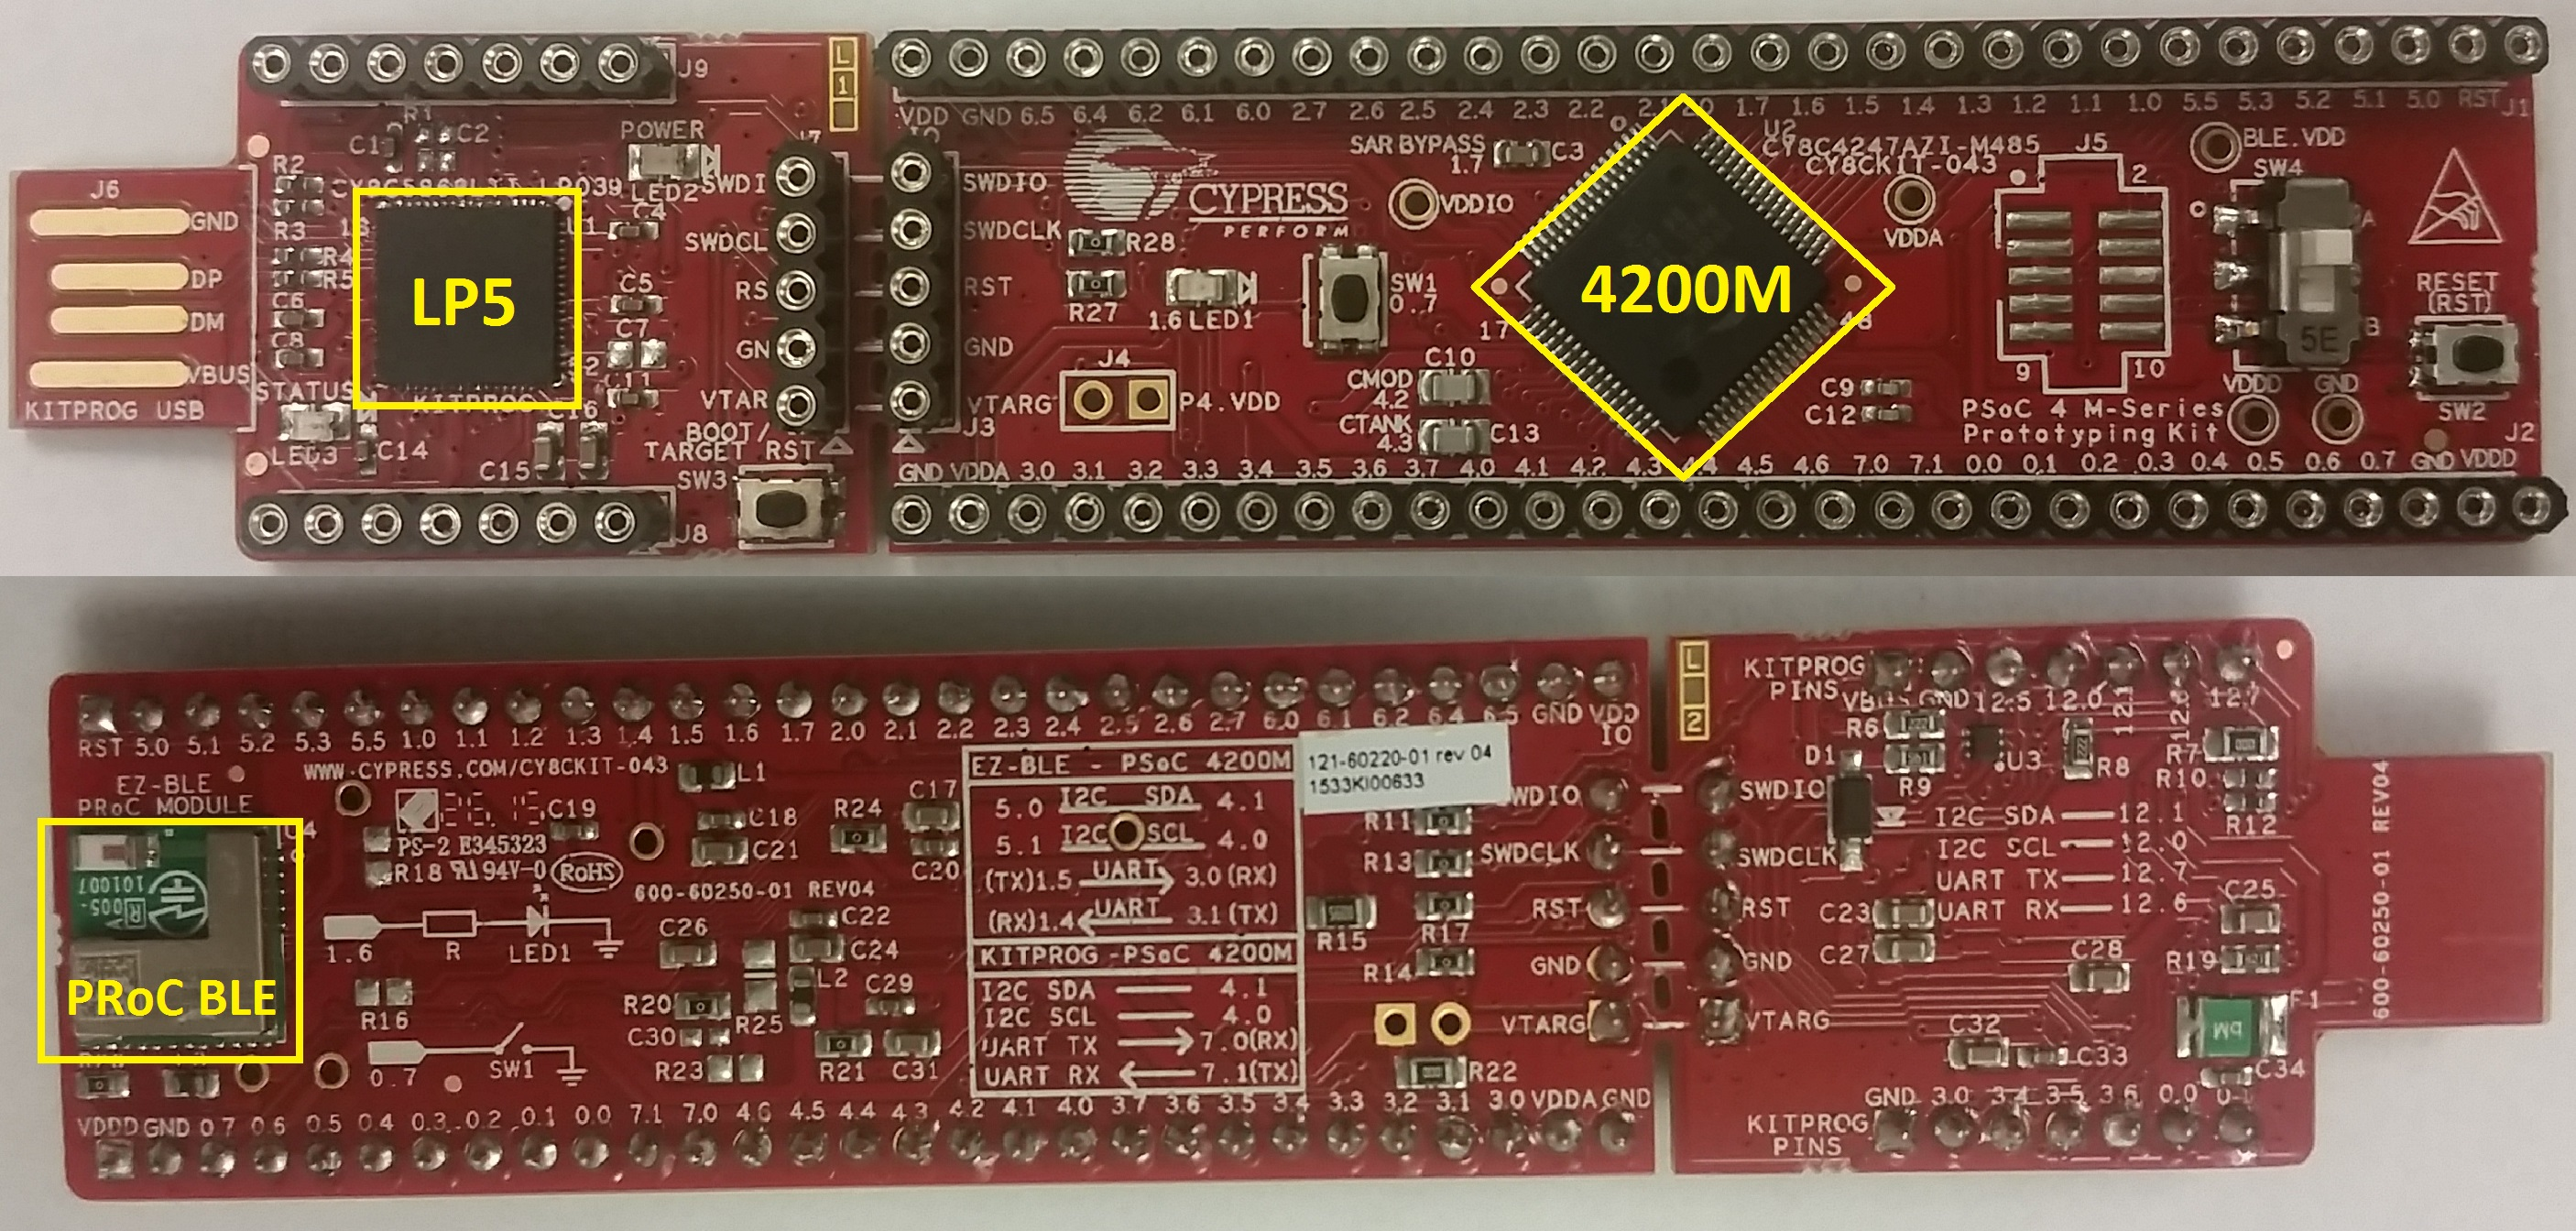
\includegraphics[scale=0.3]{figures/dProblemloesning/PSoC3.PNG}
	\caption{På figuren ses mikrokontrolleren CY8CKIT-043 PSoC 4 M-Series Prototyping Kit foran og bagpå. På forsiden findes to PSoC og på bagsiden findes PRoC, som alle er tydeliggjort med gul markering og navngivning.}
	\label{fig:PSoC}
\end{figure}

%Denne prototyping Kit platform er ved hjælp af en computer med aktiv bluetooth i stand til at sende og modtage trådløs data fra Y8CKIT-042-BLE Bluetooth® Low Energy (BLE) Pioneer Kit platformen, som indeholder en PRoC.
%CYPRESS2016BLE
%CYPRESS2016PSoC
%Semiconductor2016
%Semiconductor2016BLE